\documentclass[12pt]{report}
\usepackage[catalan]{babel}
%\usepackage[latin1]{inputenc}   % Permet usar tots els accents i car��?ters llatins de forma directa.
\usepackage[applemac]{inputenc}  
\usepackage{enumerate}
\usepackage{amsfonts, amscd, amsmath, amssymb}
\usepackage[pdftex]{graphicx}

\setlength{\textwidth}{16cm}
\setlength{\textheight}{24.5cm}
\setlength{\oddsidemargin}{-0.3cm}
\setlength{\evensidemargin}{0.25cm} \addtolength{\headheight}{\baselineskip}
\addtolength{\topmargin}{-3cm}

\newcommand\Z{\mathbb{Z}}
\newcommand\R{\mathbb{R}}
\newcommand\N{\mathbb{N}}
\newcommand\Q{\mathbb{Q}}
\newcommand\K{\Bbbk}
\newcommand\C{\mathbb{C}}

\newcounter{exctr}
\newenvironment{exemple}
{ \stepcounter{exctr} 
\hspace{0.2cm} 
\textit{Exemple  \arabic{exctr}: }
\it
\begin{quotation}
}{\end{quotation}}

\pagestyle{empty}

\begin{document}

\begin{center}
\textbf{\Large Fonaments i Aplicacions del Processament Digital dels Senyals.\\ Control 1. Curs 2012-13}
\end{center}

\vskip 1cm
\noindent
Un sistema LTI es pot representar gr�ficament amb el seg�ent esquema:

\noindent
\begin{figure}[htbp]
\begin{center}
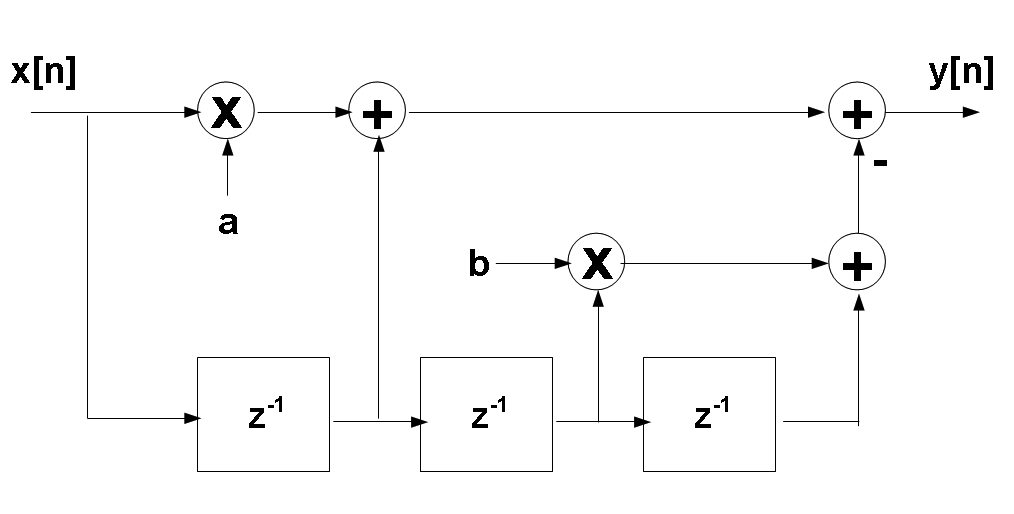
\includegraphics[width=15cm]{figuraPDScontrol1.png}
\end{center}
\end{figure}

\begin{enumerate}[a)]
\item Trobau la f�rmula que relaciona l'entrada i la sortida del sistema.
\item Comprovau que es tracta d'un sistema LTI.
\item Calculau la resposta impulsional del sistema i representau-la gr�ficament per al cas $a=2$ i $b=3$.
\item �s un sistema causal? �s un sistema estable? Justificau les respostes.
\item Utilitzau l'operaci� de convoluci� per trobar la resposta del sistema a l'esgla� unitari $u[n]$ en el cas $a=2$ i $b=3$.
\end{enumerate}




\end{document}